\documentclass[aspectratio=169]{beamer}

\usetheme{Madrid}
\usecolortheme{seagull}
\setbeamertemplate{navigation symbols}{}

\usepackage[utf8]{inputenc}
\usepackage[T1]{fontenc}
\usepackage{lmodern}
\usepackage{amsmath, amssymb}
\usepackage{booktabs}
\usepackage{array}
\usepackage{graphicx}
\usepackage{siunitx}
\usepackage{hyperref}
\usepackage{tikz}
\usetikzlibrary{arrows.meta,positioning,shapes.geometric}
\usepackage{qrcode}
\usepackage{animate} % For playing animations directly

\title[Diffeomorphic Learning]{Diffeomorphic Learning for Nonlinear Classification}
\subtitle{Revising the Mathematical Flow, Geometry, \& Numerical Results}
\author{Final Presentation }
\date{\today}

\begin{document}

\begin{frame}
  \titlepage
\end{frame}

\begin{frame}{Agenda}
\tableofcontents
\end{frame}

\section{Motivation and Introduction}

\begin{frame}{Motivation}
\textbf{Core objective:} Learn a smooth global deformation that makes difficult, non-linearly separable classification problems simpler for a final linear model.

\vspace{2mm}
\textbf{Why this matters:}
\begin{itemize}
  \item Many datasets are topologically bound and not linearly separable in their original geometry.
  \item Deep black-box nonlinear models can be accurate but less interpretable.
  \item Diffeomorphic learning provides an explicit, invertible geometric transformation governed by physical energy constraints.
\end{itemize}

\textbf{Classifier form:}
\[
 x \mapsto F(\phi(x);\theta).
\]
\end{frame}






\begin{frame}{Introduction: Geometric Learning View}
\begin{itemize}
  \item $\phi$ is a \textbf{diffeomorphism}: smooth, invertible, and topology-preserving.
  \item The model moves training samples through a smooth, time-dependent flow (velocity field) to improve separability without tearing the space.
  \item A simple terminal classifier (e.g. logistic regression) is subsequently applied.
\end{itemize}

\vspace{2mm}
\textbf{Design principle (The Trade-Off):}
\begin{itemize}
  \item Maximize final prediction accuracy.
  \item Minimize the complexity (i.e., the physical kinetic energy) of the topological deformation.
\end{itemize}
\end{frame}







\section{Mathematical Formulation}

\begin{frame}{Original Cost Function}
The objective balances deformation effort, model complexity, and data fit:
\[
G(\phi,\theta)= \underbrace{D(\mathrm{id},\phi)^2}_{\text{Deformation Cost}} + \underbrace{\lambda g(\theta)}_{\text{Regularization}} + \underbrace{\frac{1}{\sigma^2}\,\Gamma\big(F(\cdot;\theta),\,\phi(1)\cdot T_0\big)}_{\text{Terminal Loss}}
\]

\begin{itemize}
  \item $D(\mathrm{id},\phi)^2 = \inf_v \int_0^1 \|v(t)\|_V^2\,dt$: In Riemannian geometry, distance is the shortest path (an $L^1$ length). However, minimizing this $L^2$ action (which physically mirrors \textbf{Kinetic Energy} $\propto \int v^2$) mathematically guarantees the exact same shortest path, but forces a smooth, constant-speed flow.
  \item $g(\theta)$: Standard regularization (e.g., $L^2$) on terminal classifier parameters $\theta$.
  \item $\Gamma$: Cross-entropy data loss that is evaluated \textbf{strictly} and only at the final time $t=1$, assessing how linearly separable the points $\phi(1)\cdot x$ have become.
\end{itemize}
\end{frame}






\begin{frame}{Kernels and the Function Space ($V$)}
The velocity field $v(t, x)$ at any time $t$ lives in a \textbf{Reproducing Kernel Hilbert Space (RKHS)} defined by a kernel $K(x,y)$.

\textbf{Choices of Kernels matter theoretically:}
\begin{itemize}
  \item \textbf{Gaussian RBF:} Smooth ($C^\infty$) transformations.
  \item \textbf{Matérn Kernels:} Highly valuable theoretically as they are equivalent to Sobolev spaces, allowing control over exact differentiability classes ($C^k$).
  \item \textbf{Graph-Based Kernels:} Used if the data resides on strict grids or defined graphs (breaking isotropic symmetries).
\end{itemize}
\end{frame}

\begin{frame}{Affine Transformations: A Theoretical Necessity}
\textbf{The Limitation of pure RKHS:}
\begin{itemize}
  \item RKHS kernels (like Gaussians) vanish at infinity. This means the model struggles to perform simple translations and rigid global rotations.
\end{itemize}

\textbf{The Fix (Section 4.3):}
\begin{itemize}
  \item We explicitly construct an extended vector space: $\widehat{v}(t, \cdot) = g(t, \cdot) + v(t, \cdot)$, where $g$ belongs to a Lie algebra (e.g., Affine transforms).
  \item \textbf{Crucial Result:} This breaks the rotational invariance of scalar kernels and massively increases the topological expressivity of the model. It is a structural necessity.
\end{itemize}
\end{frame}



\begin{frame}{How to Optimize? The Kernel Trick \& Control Points}
Optimizing an infinite-dimensional flow $v(t)$ is impossible numerically.

\vspace{1mm}
\textbf{The RKHS Reduction:}
Because the end-loss only depends on the trajectories of the $N$ sample points, the Representer theorem guarantees the optimal velocity takes the finite form:
\[
v(t,\cdot)=\sum_{k=1}^{N} K\big(\cdot,z_k(t)\big) a_k(t)
\]

We have transformed an infinite-dimensional problem into finding \textbf{finite, time-dependent control vectors} $a_k(t)$ attached to the traveling points $z_k(t)$.
\end{frame}




\begin{frame}{The Complete Reduced Optimal Control Problem}
When we include the Affine transformation $g(t, x) = A(t)x + b(t)$, the total velocity field becomes:
\[
\widehat{v}(t,\cdot) = g(t,\cdot) + \sum_{k=1}^{N} K\big(\cdot,z_k(t)\big) a_k(t)
\]

Plugging this back into our original cost formulation yields our final \textbf{computable} objective:
\[
\mathcal{E}(a, g, \theta) = \underbrace{\int_0^1 \|g(t)\|_{\mathfrak{a}}^2 \,dt}_{\text{Affine Energy}} + \underbrace{\int_0^1 \sum_{k,l} a_k(t)^T K(z_k(t), z_l(t)) a_l(t) \,dt}_{\text{RKHS Energy}} + \lambda g(\theta) + \frac{1}{\sigma^2}\Gamma
\]

\vspace{1mm}
\textbf{The updated flow constraints:}
\[
\dot{z}_k(t) = \widehat{v}\big(t, z_k(t)\big), \quad z_k(0) = x_k
\]

This completely reduces the continuous setting to an exact \textbf{finite-dimensional optimal control problem} over variables $a, g,$ and $\theta$.
\end{frame}

\begin{frame}{Pontryagin Maximum Principle: Why Applicable Here}
We have exactly the PMP setting:
\begin{itemize}
  \item State equation (ODE) driven by continuous controls $a(t)$.
  \item Integral running cost + terminal loss evaluated at $t=1$.
  \item Smooth dynamics and differentiable objective.
\end{itemize}

Hence, first-order optimality can be characterized via a \textbf{Hamiltonian mechanics} system coupling the forward positions with a backward co-state $p(t)$.

\vspace{2mm}
\textbf{Role in practice:} PMP mechanics naturally provide the exact \textbf{Backpropagation-Through-Time (BPTT)} equations needed to iteratively extract gradients.
\end{frame}

\begin{frame}{Applying PMP: Continuous Optimality System}
Define Hamiltonian (control form):
\[
H_a(p,z)=\langle p, f(z,a)\rangle - L(z,a),
\]
with the drift defined by the RKHS kernel:
\[
f_k(z,a)=\sum_l K(z_k,z_l)a_l.
\]

\textbf{PMP conditions (The physics of the flow):}
\[
\dot z = \partial_p H_a \quad \text{(Data flows forward)}, \qquad
\dot p = -\partial_z H_a \quad \text{(Error flows backward)}.
\]

\textbf{Boundary condition (Terminal gradient at $t=1$):}
\[
p(1)=\frac{1}{\sigma^2}\,\partial_z\Gamma\big(F(\cdot;\theta),T(z(1))\big).
\]
\end{frame}

\begin{frame}{Discretized Final Formula (Used Numerically)}
\textbf{Euler discretization} ($t=0,\dots,T-1$):
\[
z(t+1)=z(t)+\frac{1}{T}\,\partial_p H_a(t).
\]
\textbf{Adjoint recursion (BPTT)}:
\[
p(t-1)=p(t)+\frac{1}{T}\,\partial_z H_a(t),
\quad
p(T-1)=\frac{1}{\sigma^2}\partial_z\Gamma.
\]
\textbf{Gradient form used in updates (for Adam/CG)}:
\[
u_k(t)=\sum_l K\big(z_k(t),z_l(t)\big)\big(p_l(t)-2a_l(t)\big).
\]

\end{frame}

\section{The Core Geometric Trick: Adding a Dimension}

\begin{frame}{Overcoming the Topology Barrier }
\textbf{The Problem:}
\begin{itemize}
  \item Diffeomorphisms are strictly topology-preserving.
  \item In 1D, this strictly means \textbf{preserving monotonicity} (a line cannot fold over itself). In $N$-D, it means points maintain their neighborhood structure without tearing or gluing space.
  \item If Class A (inner circle) is completely surrounded by Class B (outer ring), \textbf{no strictly 2D diffeomorphism can separate them} without tearing the space!
\end{itemize}

\textbf{The Theoretical Solution (Lifting / The Dummy Dimension):}
\begin{itemize}
  \item Adding a dummy dimension is one structural solution proposed within this framework to resolve the topological restriction.
  \item We augment our data with an extra coordinate: $x \to (x, 0)$.
  \item In this $(d+1)$-dimensional space, the topological barrier is broken. The velocity field simply lifts Class A \textbf{over} or \textbf{under} Class B in the dummy dimension, flattening them out perfectly for logistic regression.
\end{itemize}
\end{frame}

\section{Computational Challenges}

\begin{frame}{Scalability and Limits}
\small
\begin{tabular}{p{3.1cm}p{4.7cm}p{5.4cm}}
\toprule
Method & Typical Complexity & Practical impact \\
\midrule
Diffeomorphic Learning & $\mathcal{O}(T d N^2)$ / iter & Main bottleneck: $N^2$ kernel coupling prevents scaling natively. \\
Logistic Regression & $\mathcal{O}(N d C)$ / iter & Very fast; strong on near-linear data. \\
Kernel SVM & $\mathcal{O}(N^3)$ & Strong nonlinear baseline but expensive at scale. \\
MLP & $\mathcal{O}(N d h)$ / epoch & Scales well linearly with minibatching. \\
\bottomrule
\end{tabular}

\vspace{2mm}
\textbf{Proposed speedups to bypass $N^2$ coupling:}
\begin{itemize}
  \item \textbf{Control points} ($n\ll N$): Represent flow with sparse landmarks instead of sample points.
  \item \textbf{Mini-batch data term}: Made possible once the control representation is decoupled from $N$, enabling stochastic gradient descent.
  \item \textbf{Parametric Models }: Replace the exact RKHS representation with a neural-net-like parametric form (e.g., $v(t,x) = \sigma(A(t)x + b(t))$), mapped over finite dimensions.
\end{itemize}
\end{frame}

\section{Numerical Tours and Results}

\begin{frame}{Experimental Setup}
\begin{itemize}
  \item \textbf{Datasets evaluated}:
    \begin{itemize}
      \item \textbf{Circles}: Concentric structures evaluating strict topological inclusion constraints.
      \item \textbf{Moons}: Intertwined geometries assessing highly non-linear boundary separation capabilities.
      \item \textbf{Blobs}: Linearly separated gaussian target clusters.
      \item \textbf{Gaussian Quantiles}: Strongly nested, dense concentric groupings testing complex boundary extraction.
    \end{itemize}
  \item \textbf{Framework Variants}: 2D baseline versus 3D Lifting strategy (employing a dummy dimension initialized with Gaussian perturbation $\sigma=0.01$).
  \item \textbf{Evaluation Environment}: Metrics reported as the test classification accuracy over 3 invariant initialized seed states.
\end{itemize}
\end{frame}

\begin{frame}{Performance: 2D vs 3D Across Datasets}
\centering
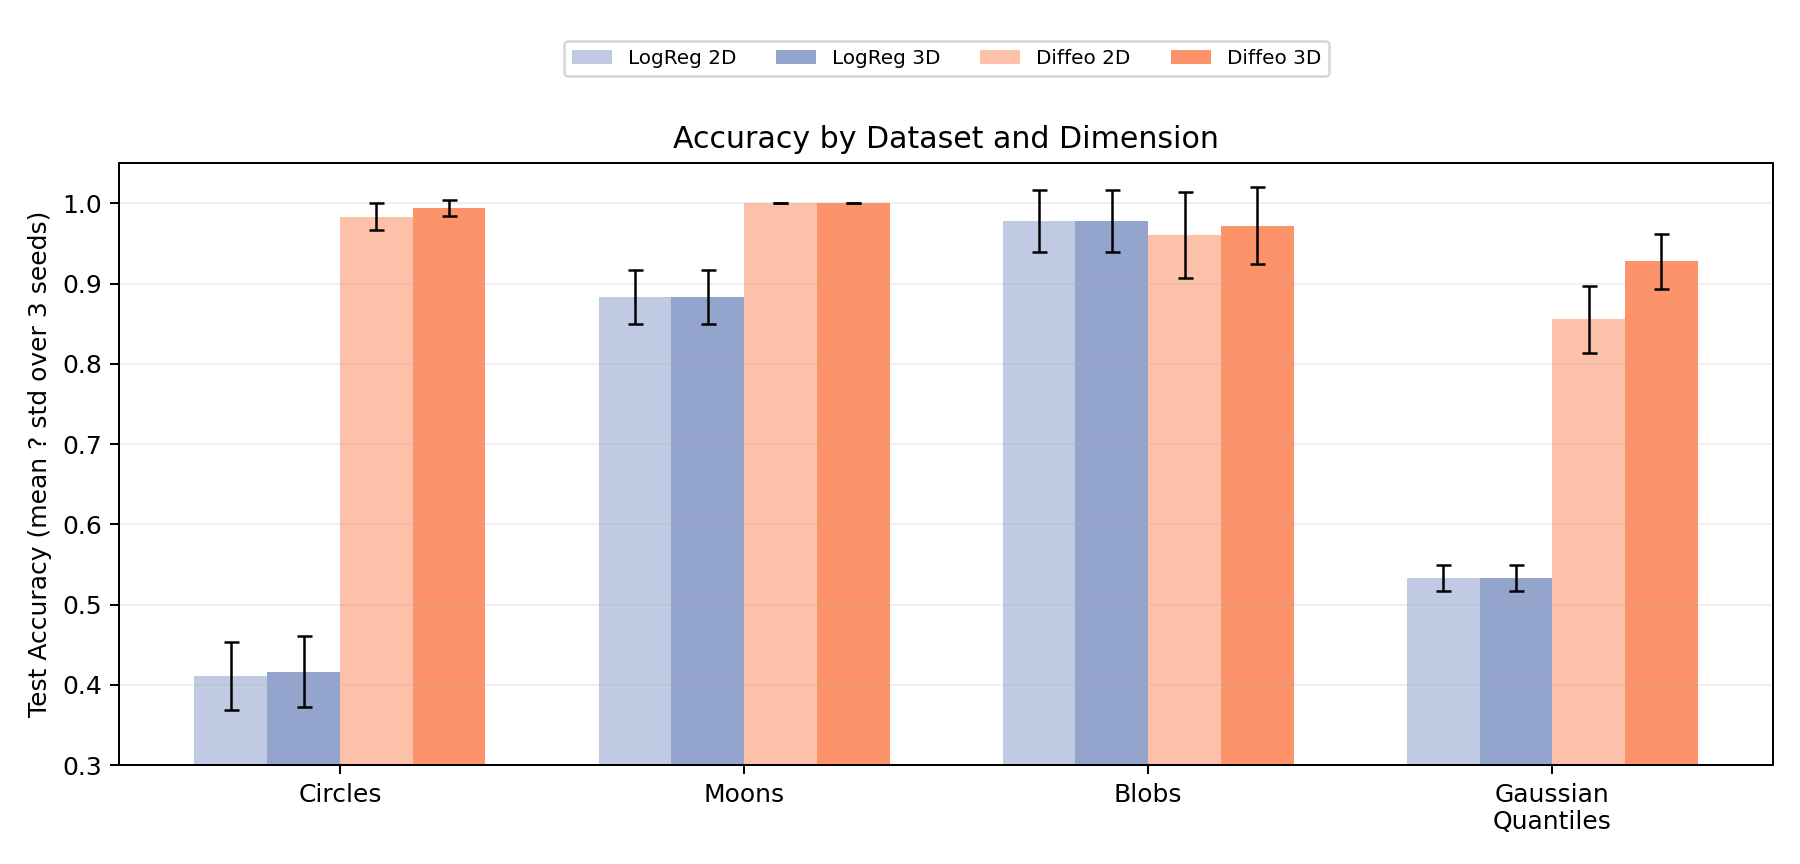
\includegraphics[width=0.95\linewidth]{four_datasets_accuracy_grouped.png}

\vspace{1mm}
\footnotesize
Notice the massive accuracy spike on Gaussian quantiles explicitly because of 3D Lifting!
\end{frame}

\begin{frame}{Results Analysis (Final Accuracy Criterion)}
\small
\centering
\begin{tabular}{lccccc}
\toprule
Dataset & LogReg 2D & LogReg 3D & Diffeo 2D & Diffeo 3D & $\Delta$ Diffeo \\
\midrule
Circles & 0.411 & 0.417 & 0.983 & 0.994 & \textbf{+0.011} \\
Moons & 0.883 & 0.883 & 1.000 & 1.000 & +0.000 \\
Blobs & 0.978 & 0.978 & 0.961 & 0.972 & +0.011 \\
Quantiles & 0.533 & 0.533 & 0.856 & 0.928 & \textbf{+0.072} \\
\bottomrule
\end{tabular}

\vspace{2mm}
\footnotesize
\begin{itemize}
  \item \textbf{Circles}: Represents a bounded topological barrier. The algorithm leverages 3D lifting to perfectly decouple the locked ring without local minima penalties.
  \item \textbf{Moons}: Devoid of strict inner boundaries. The native 2D continuous flow unbends the intertwined distribution seamlessly, achieving absolute precision accuracy universally.
  \item \textbf{Blobs}: Natively linearly separable configurations. Diffeomorphic routing performs similarly to native linear limits across configurations with standard negligible deviation.
  \item \textbf{Gaussian Quantiles}: The ultimate test for topological lifting, holding distinct intersecting rings. 3D projection mathematically acts as the essential variable enabling internal boundaries to elevate over exterior clusters resulting in the definitive $7.2\%$ accuracy climb.
\end{itemize}
\end{frame}


\begin{frame}{Results Analysis: Circles Dataset (2D Flow)}
\begin{columns}
\begin{column}{0.5\textwidth}
\centering
\textbf{Before} \\
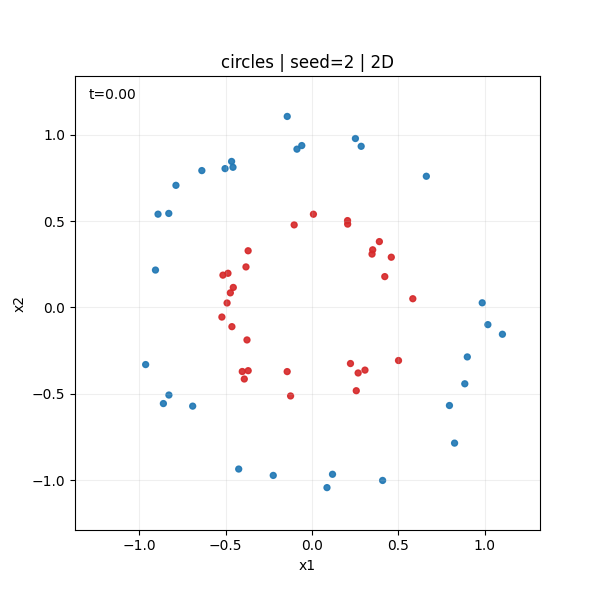
\includegraphics[width=0.85\textwidth]{animacoes/frames/circles_2D_frames/before.png}
\end{column}
\begin{column}{0.5\textwidth}
\centering
\textbf{After} \\
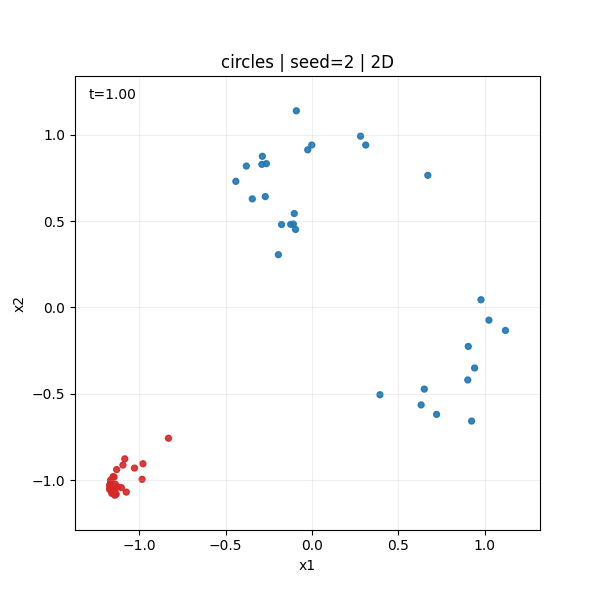
\includegraphics[width=0.85\textwidth]{animacoes/frames/circles_2D_frames/after.png}
\end{column}
\end{columns}

\vspace{5mm}
\centering \footnotesize
Native 2D deformations on the concentric Circles target. Notice the topological restriction limits complete geometric decoupling.
\end{frame}

\begin{frame}{Results Analysis: Circles Dataset (3D Lifting)}
\begin{columns}
\begin{column}{0.5\textwidth}
\centering
\textbf{Before} \\
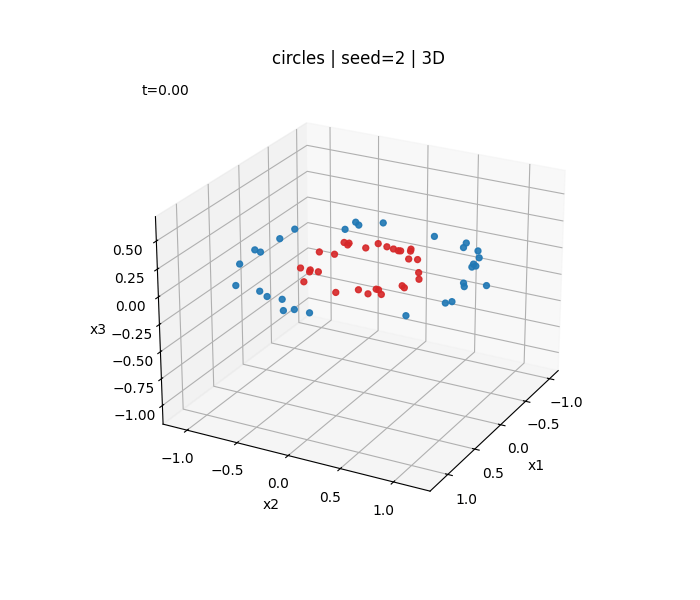
\includegraphics[width=0.85\textwidth]{animacoes/frames/circles_3D_frames/before.png}
\end{column}
\begin{column}{0.5\textwidth}
\centering
\textbf{After} \\
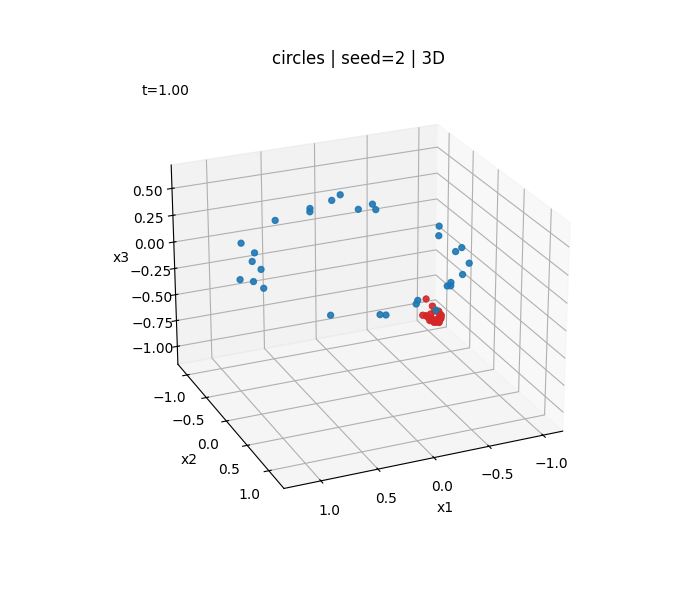
\includegraphics[width=0.85\textwidth]{animacoes/frames/circles_3D_frames/after.png}
\end{column}
\end{columns}

\vspace{5mm}
\centering \footnotesize
By injecting a 3D dummy dimension, the model correctly separates the locked ring over the surrounding context, reaching near 100\% metric convergence.
\end{frame}

\begin{frame}{Results Analysis: Moons Dataset (2D Flow)}
\begin{columns}
\begin{column}{0.5\textwidth}
\centering
\textbf{Before} \\
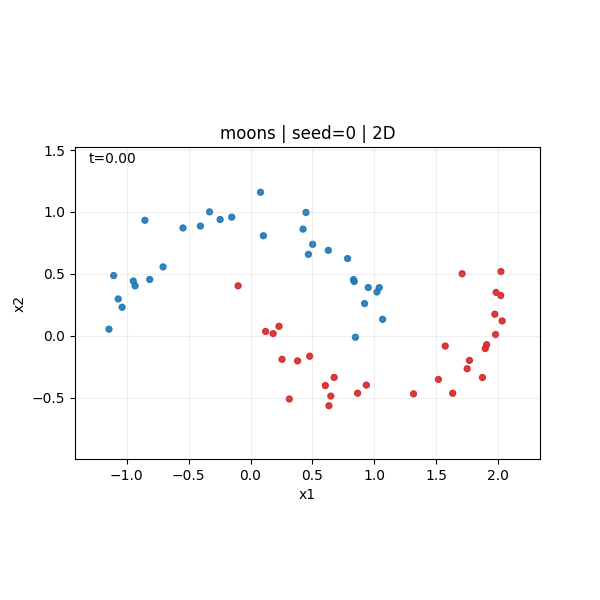
\includegraphics[width=0.85\textwidth]{animacoes/frames/moons_2D_frames/before.png}
\end{column}
\begin{column}{0.5\textwidth}
\centering
\textbf{After} \\
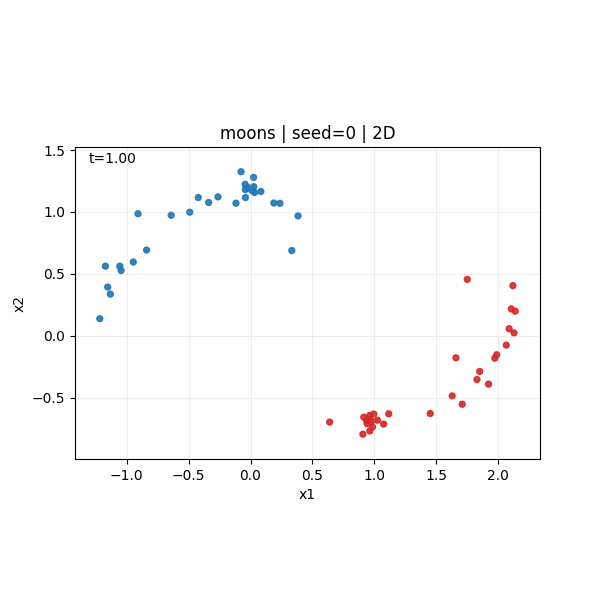
\includegraphics[width=0.85\textwidth]{animacoes/frames/moons_2D_frames/after.png}
\end{column}
\end{columns}

\vspace{5mm}
\centering \footnotesize
2D spatial deformations successfully unbending the intertwined Moons distributions since they are not bounded continuously.
\end{frame}

\begin{frame}{Results Analysis: Moons Dataset (3D Lifting)}
\begin{columns}
\begin{column}{0.5\textwidth}
\centering
\textbf{Before} \\
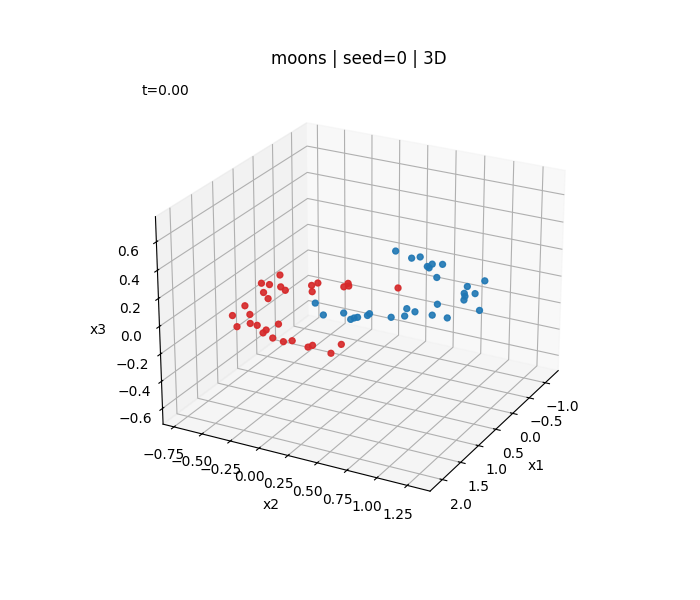
\includegraphics[width=0.85\textwidth]{animacoes/frames/moons_3D_frames/before.png}
\end{column}
\begin{column}{0.5\textwidth}
\centering
\textbf{After} \\
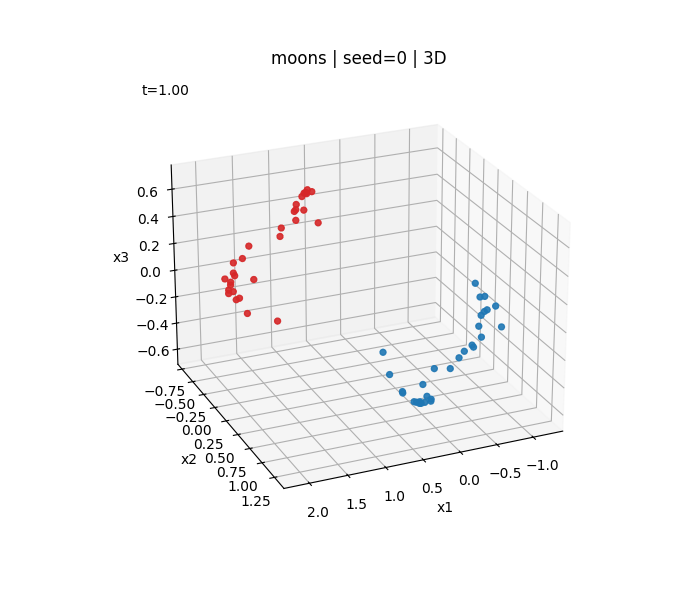
\includegraphics[width=0.85\textwidth]{animacoes/frames/moons_3D_frames/after.png}
\end{column}
\end{columns}

\vspace{5mm}
\centering \footnotesize
3D Lifting results for the Moons dataset; minimal dimensional gain is noted since the 2D plane flow already achieved full accuracy.
\end{frame}

\begin{frame}{Results Analysis: Blobs Dataset (2D Flow)}
\begin{columns}
\begin{column}{0.5\textwidth}
\centering
\textbf{Before} \\
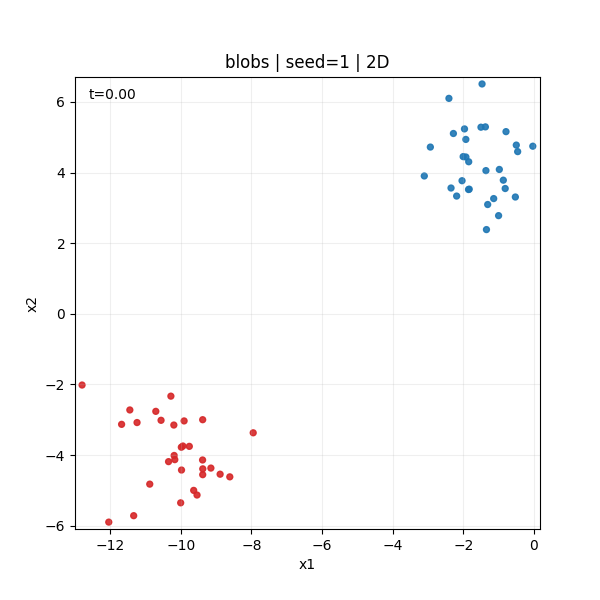
\includegraphics[width=0.85\textwidth]{animacoes/frames/blobs_2D_frames/before.png}
\end{column}
\begin{column}{0.5\textwidth}
\centering
\textbf{After} \\
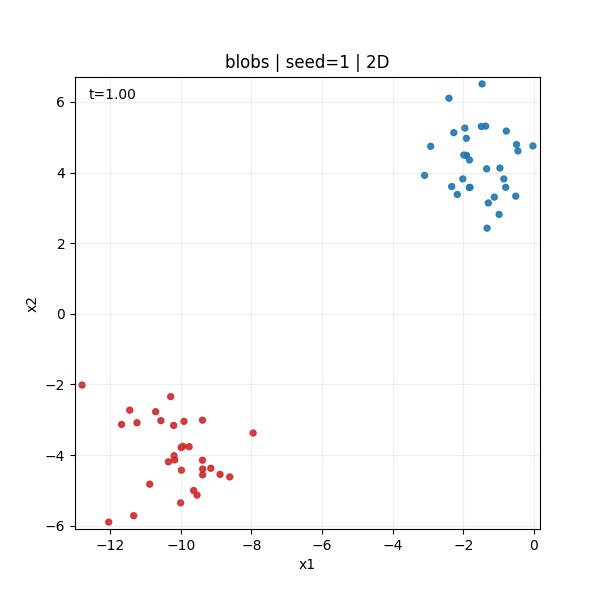
\includegraphics[width=0.85\textwidth]{animacoes/frames/blobs_2D_frames/after.png}
\end{column}
\end{columns}

\vspace{5mm}
\centering \footnotesize
Basic alignment of linearly separable Gaussian Blobs via learned 2D mapping.
\end{frame}

\begin{frame}{Results Analysis: Blobs Dataset (3D Lifting)}
\begin{columns}
\begin{column}{0.5\textwidth}
\centering
\textbf{Before} \\
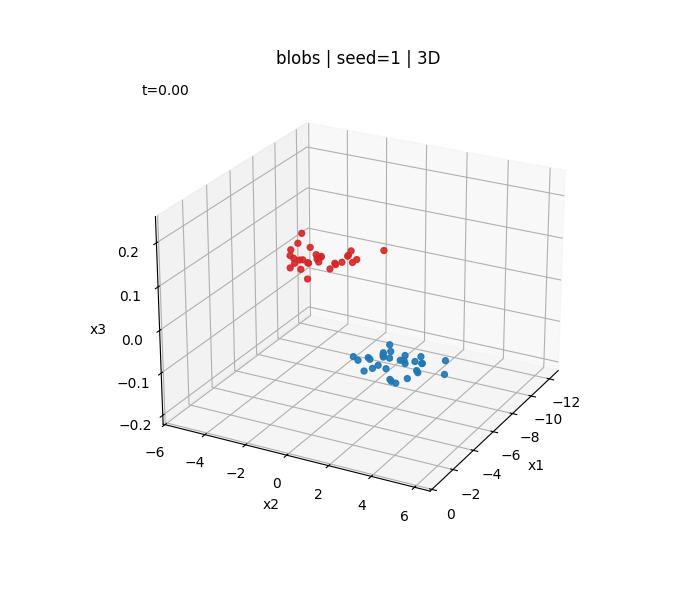
\includegraphics[width=0.85\textwidth]{animacoes/frames/blobs_3D_frames/before.png}
\end{column}
\begin{column}{0.5\textwidth}
\centering
\textbf{After} \\
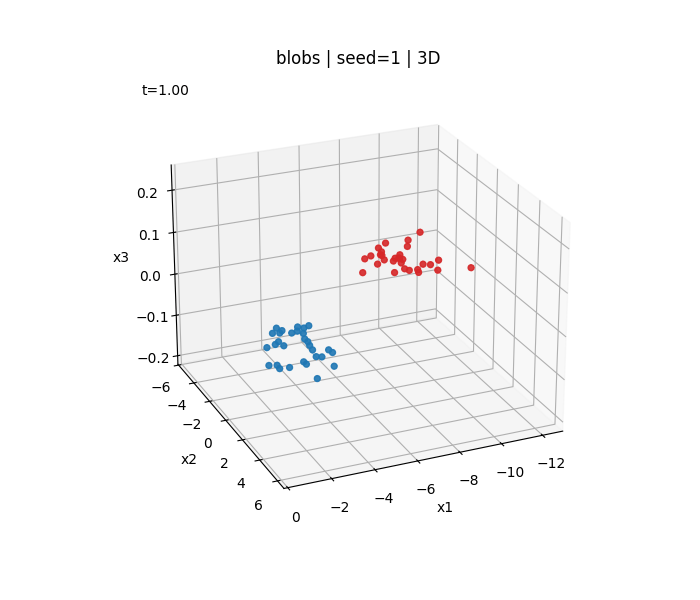
\includegraphics[width=0.85\textwidth]{animacoes/frames/blobs_3D_frames/after.png}
\end{column}
\end{columns}

\vspace{5mm}
\centering \footnotesize
Dummy coordinate lifting over previously separated Blobs; Diffeomorphic models collapse seamlessly to simple affine transforms here.
\end{frame}

\begin{frame}{Results Analysis: Gaussian Quantiles (2D Flow)}
\begin{columns}
\begin{column}{0.5\textwidth}
\centering
\textbf{Before} \\
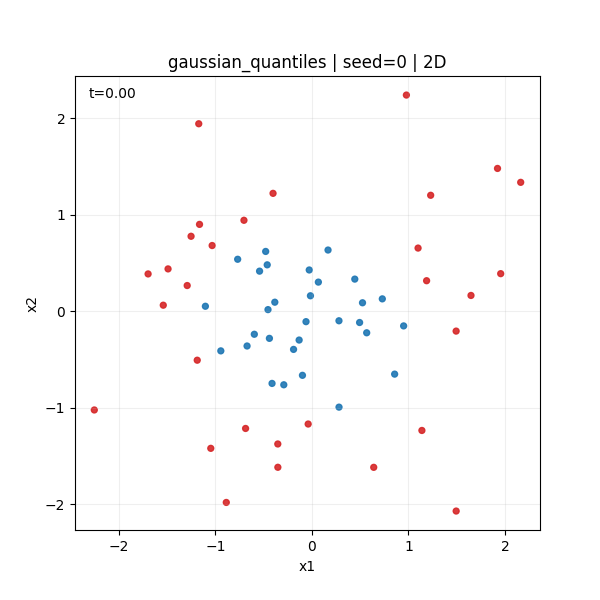
\includegraphics[width=0.85\textwidth]{animacoes/frames/gaussian_quantiles_2D_frames/before.png}
\end{column}
\begin{column}{0.5\textwidth}
\centering
\textbf{After} \\
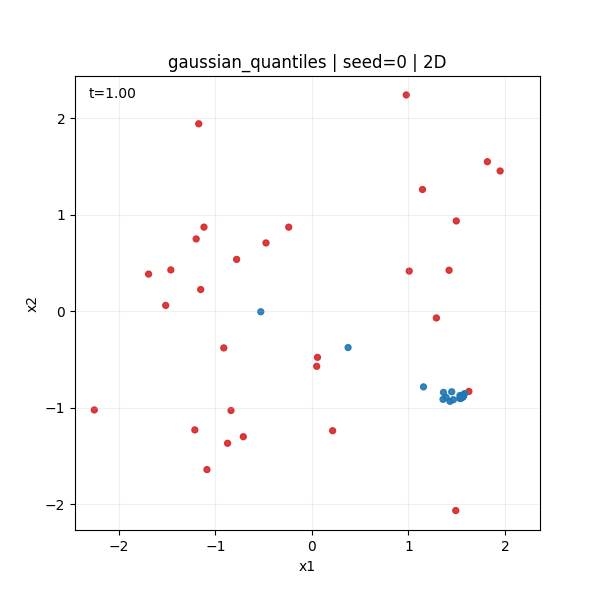
\includegraphics[width=0.85\textwidth]{animacoes/frames/gaussian_quantiles_2D_frames/after.png}
\end{column}
\end{columns}

\vspace{5mm}
\centering \footnotesize
Struggling to cluster interlaced target segments inside the Quantiles dataset natively within the 2D bounding volume.
\end{frame}

\begin{frame}{Results Analysis: Gaussian Quantiles (3D Lifting)}
\begin{columns}
\begin{column}{0.5\textwidth}
\centering
\textbf{Before} \\
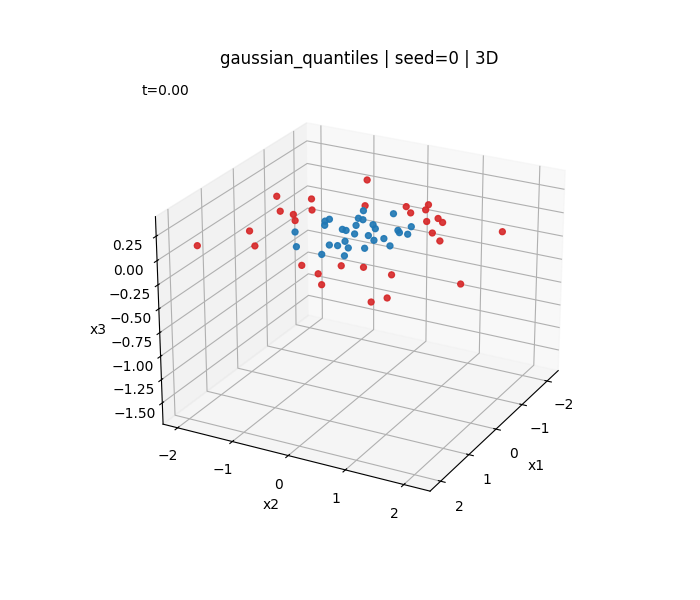
\includegraphics[width=0.85\textwidth]{animacoes/frames/gaussian_quantiles_3D_frames/before.png}
\end{column}
\begin{column}{0.5\textwidth}
\centering
\textbf{After} \\
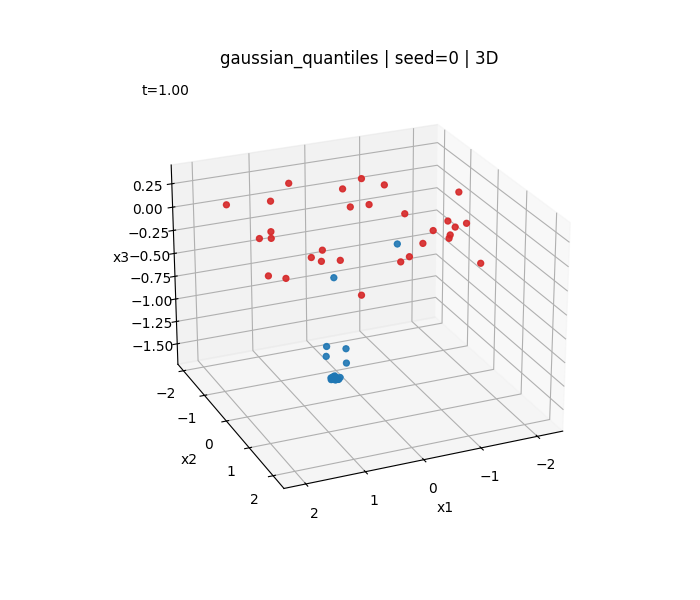
\includegraphics[width=0.85\textwidth]{animacoes/frames/gaussian_quantiles_3D_frames/after.png}
\end{column}
\end{columns}

\vspace{5mm}
\centering \footnotesize
Maximum performance climb (+7.2\% Delta): Complete spatial unlocking using the hidden vertical axis yielding a smooth, continuous topology lift over intersecting sets.
\end{frame}

\section{Implementation \& Conclusion}

\begin{frame}{Implementation Schema}
\centering
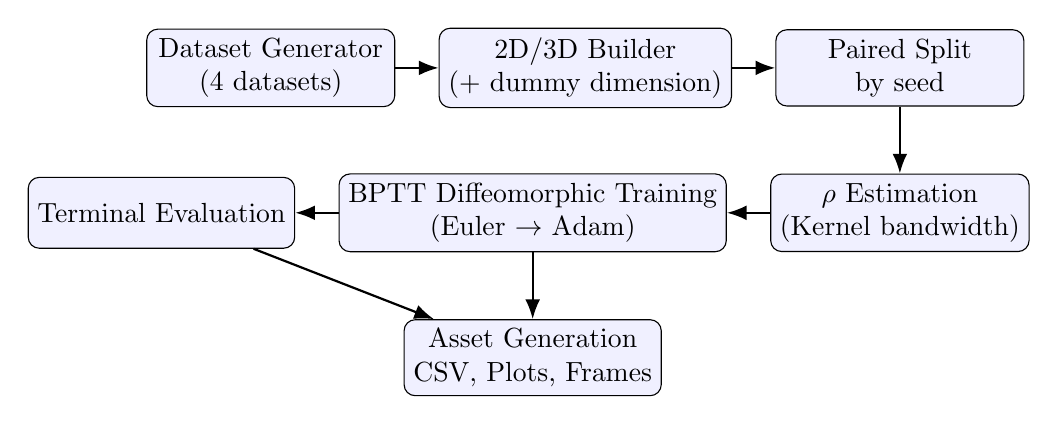
\begin{tikzpicture}[
  node distance=0.85cm and 0.55cm,
  block/.style={rectangle, rounded corners, draw=black, fill=blue!6, align=center, minimum width=3.15cm, minimum height=0.9cm},
  line/.style={-{Latex[length=2.5mm]}, thick}
]
\node[block] (data) {Dataset Generator\\(4 datasets)};
\node[block, right=of data] (lift) {2D/3D Builder\\(+ dummy dimension)};
\node[block, right=of lift] (split) {Paired Split\\by seed};
\node[block, below=of split] (rho) {$\rho$ Estimation\\(Kernel bandwidth)};
\node[block, left=of rho] (train) {BPTT Diffeomorphic Training\\(Euler $\rightarrow$ Adam)};
\node[block, left=of train] (eval) {Terminal Evaluation};
\node[block, below=of train] (out) {Asset Generation\\CSV, Plots, Frames};

\draw[line] (data) -- (lift);
\draw[line] (lift) -- (split);
\draw[line] (split) -- (rho);
\draw[line] (rho) -- (train);
\draw[line] (train) -- (eval);
\draw[line] (eval) -- (out);
\draw[line] (train) -- (out);
\end{tikzpicture}
\end{frame}

\begin{frame}{Conclusion}
\begin{itemize}
  \item \textbf{Topological Flow:} Diffeomorphic learning is a physically intuitive optimal transport model replacing the "black-box" mechanics of standard NNs.
  \item \textbf{The Core Tricks:} Incorporating Affine extensions breaks invariance, while adding a single Dummy coordinate completely solves the restriction of topological preservation.
  \item \textbf{Numerical reality:} The $O(N^2)$ explicit calculation is a heavy bottleneck; future work must concentrate on sparse parametric approximations rather than exact numerical representation.
\end{itemize}
\end{frame}

\begin{frame}
\centering
\Large Thank you.

\vspace{1cm}
\qrcode[height=3cm]{https://github.com/EwerthonMelzani/Espace-des-Formes\#}
\end{frame}

\end{document}
